\chapter{Approach}
\label{ch:experimental_analysis}

\todo[inline]{Add a short introduction to the chapter.}

\section{Empirical Analysis of Separator Scaling in Road Networks}
\label{sec:empirical_analysis}

To empirically investigate the relationship between graph size and separator size in road networks, we analyze data derived from a road network graph of Europe \cite{ptv_group_dimacs-europe_2009}.
A crucial first step in our research, addressed by this analysis, is to empirically validate whether road networks exhibit separators scaling near \(\bigO{n^{1/3}}\), as suggested by prior work \cite{dibbelt_customizable_2016}, as opposed to an alternative, like \(\bigO{n^{1/2}}\), potentially appearing smaller due to a low constant factor.
Figure \cref{fig:separator_size_vs_graph_size} plots the size of separators against the size of the corresponding subgraphs from which they were computed.
Each data point \( (x, y) \) in this figure signifies that a subgraph containing \( x \) nodes possesses a separator of size \( y \).
The dataset contains separators of subgraphs generated by a nested dissection, computing separators first for the original graph and then for the subgraphs induced at each level.

\begin{figure}
	\centering
	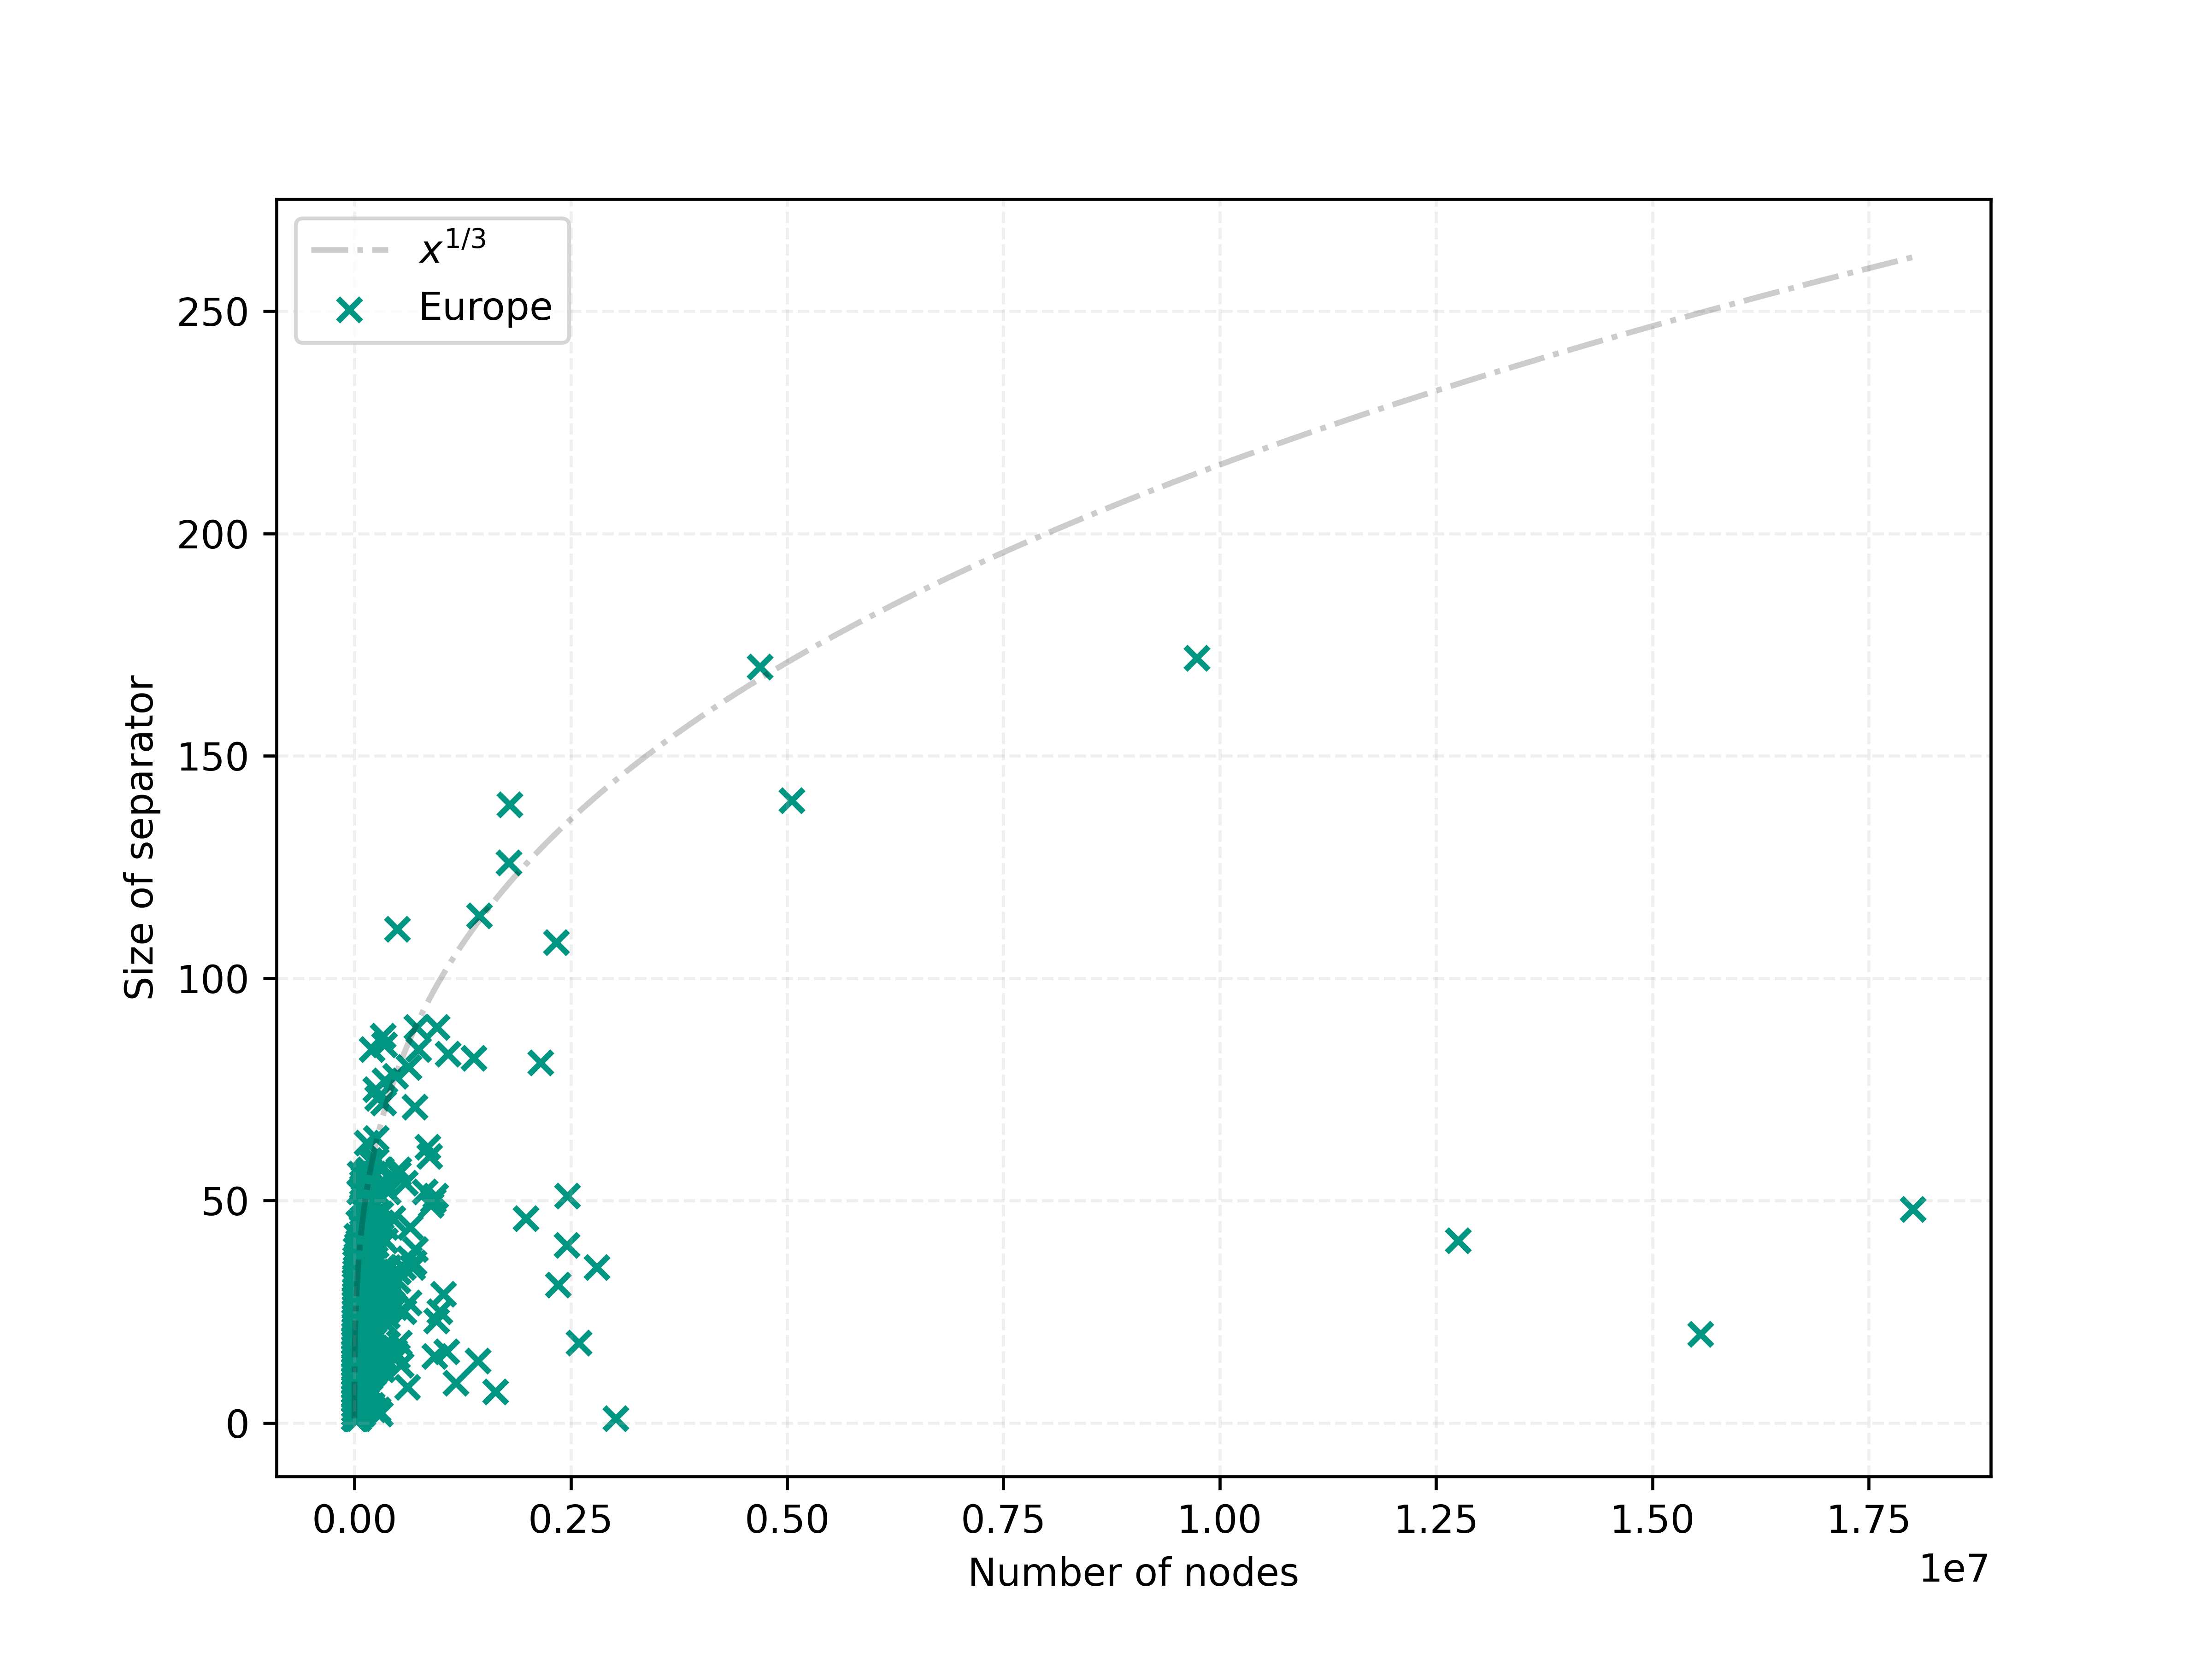
\includegraphics[width=0.7\linewidth]{graphics/Europe.png}
	\caption{Empirical separator size versus subgraph size for the Europe road network. Each point represents a subgraph and its corresponding separator size.}
	\label{fig:separator_size_vs_graph_size}
\end{figure}

Initial observations reveal outliers, particularly for very large subgraphs corresponding to continental or country scales.
Specifically, analysis of the top-level separator structure for the Europe graph shows that the Scandinavian peninsula can be disconnected via separators significantly smaller than the general trend would suggest, due to specific geographic bottlenecks.
This can be seen in \cref{fig:europe_top_separator}.
Such outliers at the largest scales appear to be heavily influenced by macroscopic geographic features rather than intrinsic network structure representative of typical road networks.
Consequently, these data points may not accurately reflect the general separator properties inherent in the finer structure of the road network graph.
To mitigate the influence of these large-scale geographical artifacts and focus on more representative structural properties, our analysis primarily considers subgraphs with fewer than 10,000,000 nodes.

\begin{figure}
	\centering
	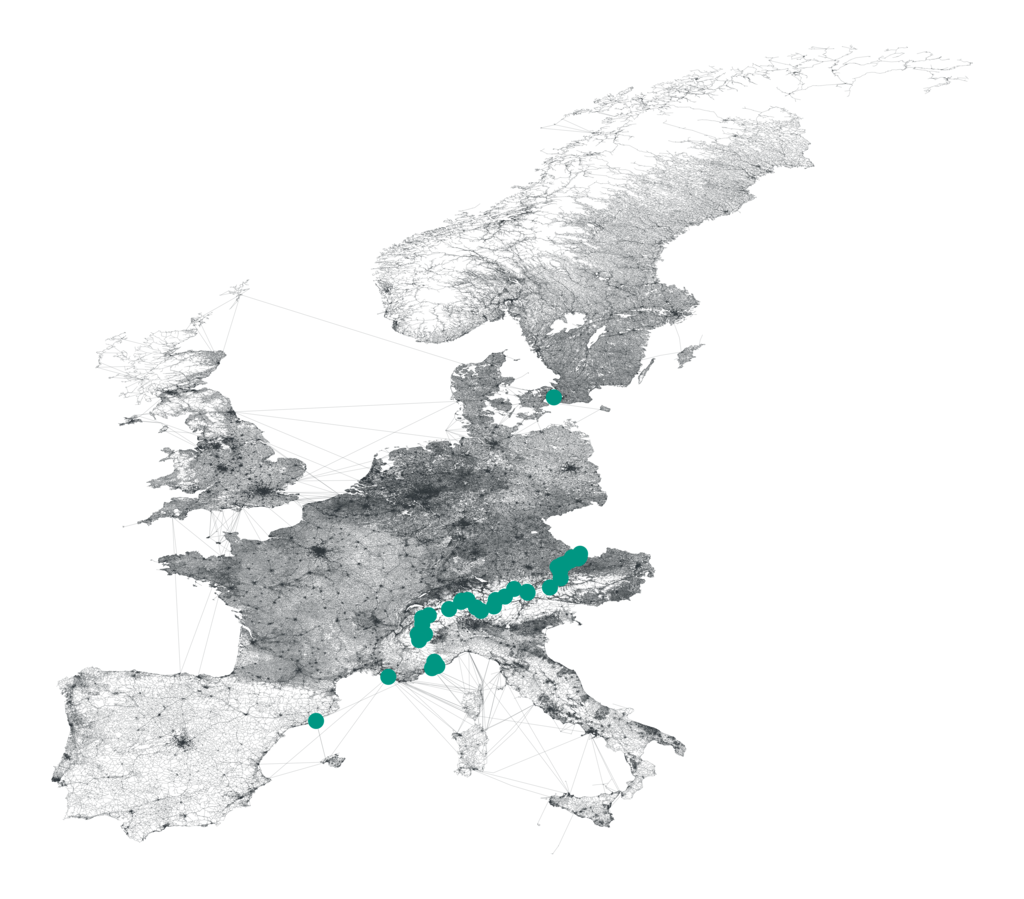
\includegraphics[width=0.6\linewidth]{graphics/europe-top-level-sep.png}
	\caption{Illustration of a geographically influenced outlier at the continental scale: removal of a few nodes disconnects the whole Scandinavian peninsula.}
	\label{fig:europe_top_separator}
\end{figure}

For enhanced visibility, particularly concerning the numerous data points corresponding to smaller subgraphs, and to avoid overrepresentation of larger subgraphs, we will also present data a log-log scale.
This logarithmic scaling offers the additional advantage that a polynomial relationship between separator size \( y \) and subgraph size \( x \), such as \( y \propto x^c \), manifests as a linear trend in the log-log plot, facilitating the identification of potential power-law dependencies.
Furthermore, to improve the interpretability of the visualization and emphasize the underlying trend over individual fluctuations or outliers present at various scales, the data points are aggregated into bins.
Let \( b \) be the number of bins chosen for the aggregation.
Let \( x_{\max} \) denote the maximum observed subgraph size, assuming \( x_{\max} > 0 \).
A data point \( (x, y) \) is assigned to the bin with index \( \floor{\frac{x \cdot b}{x_{\max}}} \).
After assigning all points to their respective bins, a single representative point is computed for each non-empty bin.
This representative point \( (\overline{x}_i, \overline{y}_i) \) for bin \( i \) is determined by calculating the arithmetic mean of the \( x \) coordinates and the arithmetic mean of the \( y \) coordinates of all data points \( (x, y) \) assigned to bin \( i \).
When constructing the log-log plot, this binning procedure is applied to the logarithmically transformed data.
\cref{fig:separator_size_loglog_binned} illustrates the binned data points on logarithmic axes.

\begin{figure}
	\centering
	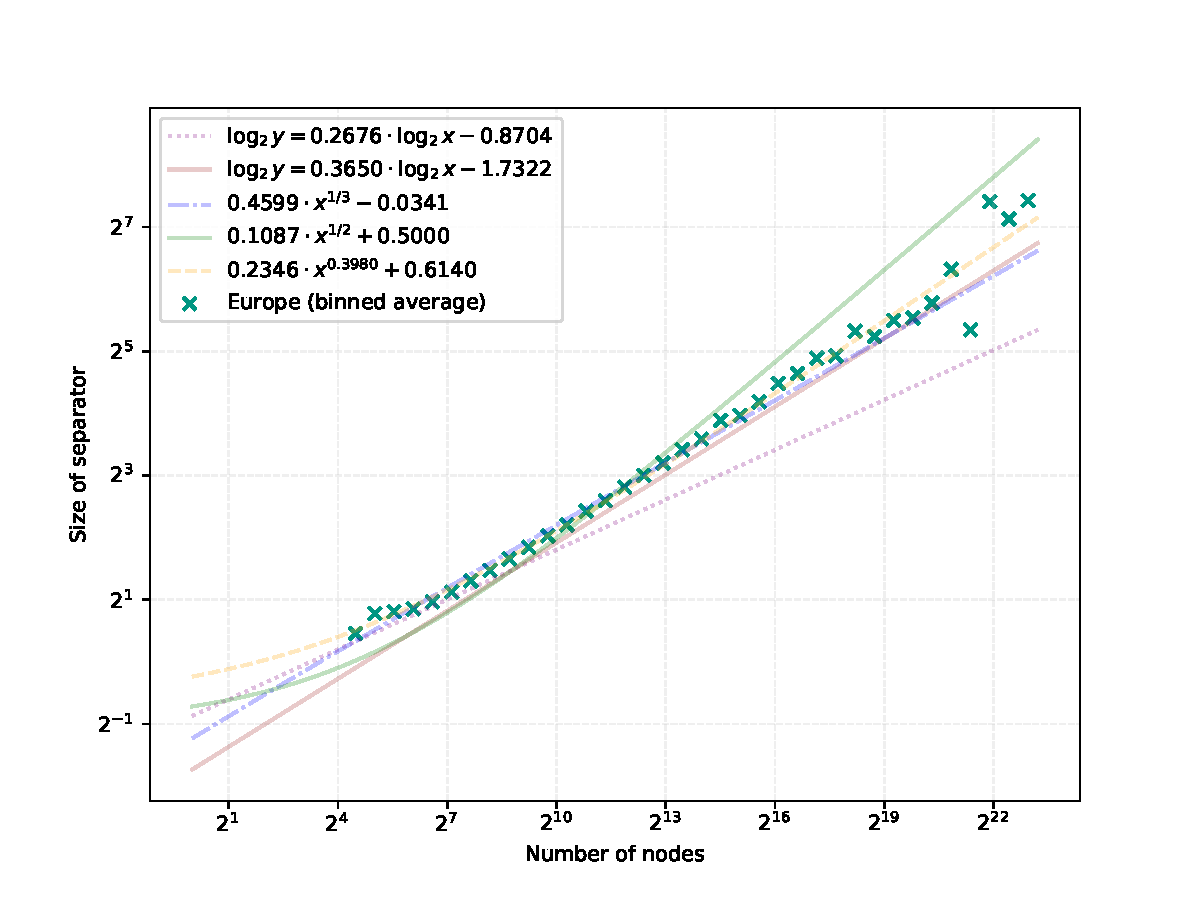
\includegraphics[width=0.7\linewidth]{graphics/Europe-binned.pdf}
	\caption{Binned separator size against subgraph size for the Europe road network on logarithmic axes (subgraphs < 10M nodes).}
	\label{fig:separator_size_loglog_binned}
\end{figure}

\todo[inline]{Add statistical analysis}

\section{Planarity} \label{sec:approach:planarity}

Road networks can be modeled as nearly planar graphs, meaning they permit embedding in the plane with a limited number of edge crossings.
Empirical evidence suggests that the number of such crossings in real-world road networks is typically in \(\Theta\!\left(n^{1/2}\right)\), where \(n\) represents the number of vertices \cite{eppstein_studying_2008}.
It is a well-known result in graph theory that planar graphs admit \(\frac23\)-balanced
separators of size \(\bigO{{n}^{1/2}}\) \cite{lipton_separator_1979}.

A relevant inquiry is whether the near-planarity of road networks is a critical
feature that influences their structural properties, or if the occasional
non-planar elements are merely incidental and do not substantially affect the
network’s overall characteristics. This prompts the question of how the
separator sizes of road networks are affected when they are transformed into
strictly planar graphs, for instance, by altering edges to eliminate crossings.

To obtain a planar representation, we begin with the existing graph structure where vertices possess associated geometric coordinates.
Each edge in this graph is interpreted as the straight line segment connecting the coordinates of its incident vertices.
The algorithm then identifies all geometric intersection points occurring between these line segments.
A new vertex is introduced into the graph at the precise coordinates of each detected intersection point, provided this point does not coincide with the coordinates of an existing endpoint of the intersecting segments.
Subsequently, any original edge that contains one or more such intersection points along its segment is removed.
It is replaced by a sequence of new, shorter edges that connect the original endpoints and the newly created intersection vertices in their linear order along the original segment.
This process transforms the initial graph into a planar graph embedding by explicitly representing edge crossings as vertices.
For efficient execution, we utilize a spatial index that stores the bounding boxes of all
edges. Under the assumption of short edges, this structure enables rapid
identification of potential intersections by querying overlapping bounding
boxes, followed by verification of actual crossings. While other algorithms
exist, such as the Bentley-Ottmann algorithm \cite{bentley_algorithms_1979},
which is designed for general segment crossings, or a linear-time algorithm
(e.g., as described in \cite{eppstein_linear-time_2010}), which is tailored for
graph structures with a sublinear number of edge crossings, we opted for this
spatial index-based approach due to its simplicity and ease of implementation,
especially since performance is not a critical concern in this context. Given
that a single edge may intersect multiple other edges, we sort the intersection
points along each edge and introduce new edges accordingly. Pseudo-code for
this planarization algorithm is provided in \cref{alg:planarization}.

\begin{algorithm}[b]
	\Input{Non-planar graph \(G=(V, E, pos)\).}
	\Output{Planarized version of \G.}
	\BlankLine
	spatial\_index \(\longleftarrow\) load(bounding\_boxes(\E))\;
	crossings \(\longleftarrow\) \{\}\;
	\ForAll{\e  in \E}{
		\ForAll{candidates \(c\) in spatial\_index.query(\e)}{
			\If{\(c\) intersects \e} {
				crossings[\(e\)].append(\(c\))\;
				crossings[\(c\)].append(\(e\))\;
			}
		}
	}
	\ForAll{(\e, crossed) in crossings}{
		\G.remove(\e)\;
		vertices \(\longleftarrow\) get\_intersection\_vertices(\(e\), crossed)\;
		sort vertices along \e\;
		add\_new\_edges(\(e\), vertices)\;
	}
	\caption{Simple planarization algorithm \label{alg:planarization}}
\end{algorithm}

We applied this planarization method to real-world road networks.
The Karlsruhe network, with approximately 120,000 nodes, revealed around 2,500 intersections.
The Germany network, comprising about 6 million nodes, exhibited approximately 100,000 intersections.
Finally the Europe network, with around 18 million nodes, contained about 300,000 intersections.
These numbers exceed the \bigO{n^{1/2}} intersection counts reported
in prior studies but remain within a similar magnitude
\cite{eppstein_studying_2008}. The differences could be explained by the
unoptimal linear assumption of edges and might be mitigated by using a more
modeled road network like OpenStreetMap.

Analysis of separator sizes showed minimal variation post-planarization. We
identified \(\frac{2}{3}\)-balanced separators of size approximately
\bigO{n^{ 1/3 }}, aligning with the values from non planar graphs. A comparison of
the separator sizes in the planar and non-planar versions of the Germany
network is depicted in \cref{fig:germany_planar_vs_non_planar}.

\begin{figure}
	\centering
	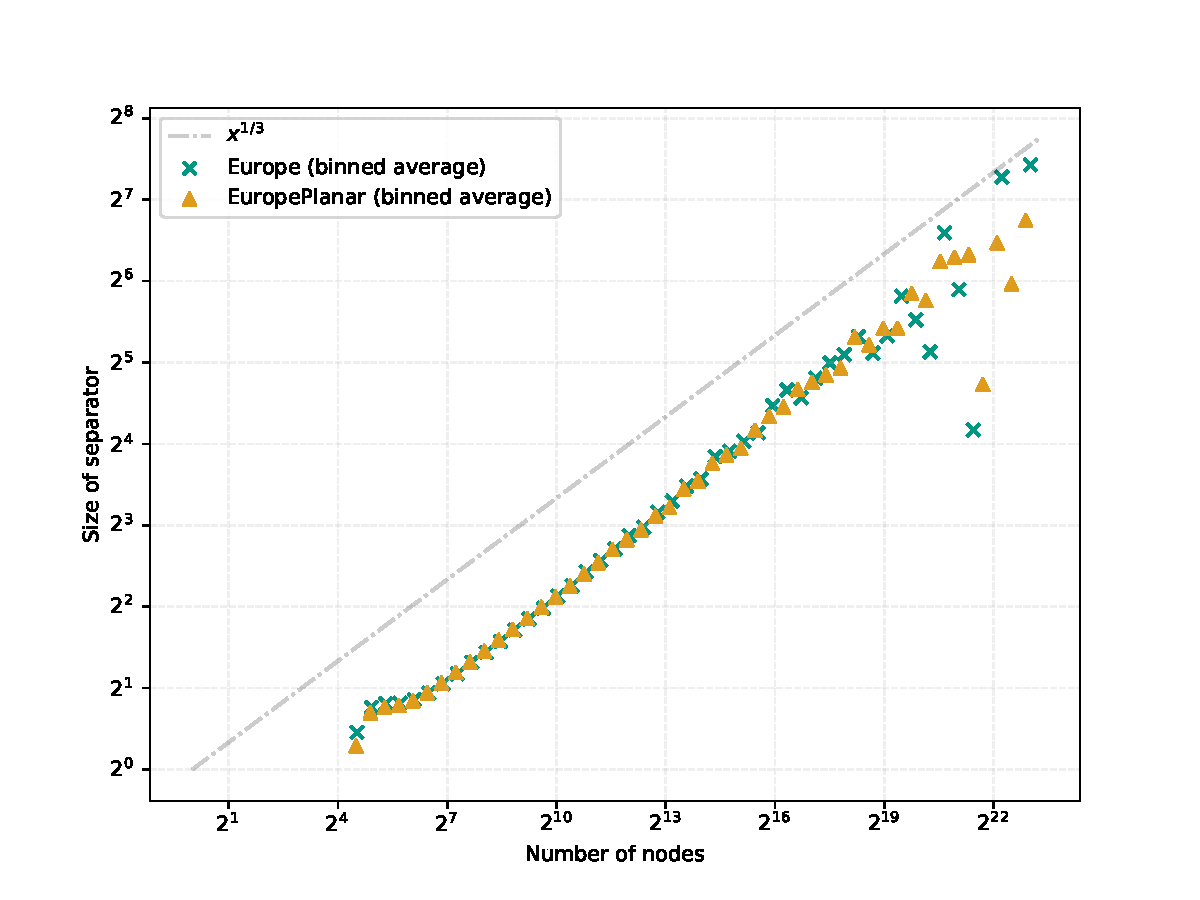
\includegraphics[width=0.8\linewidth]{graphics/EuropePlanarVsNonPlanar.pdf}
	\caption{Comparison of separator sizes in the European road network: planar vs. non-planar.}
	\label{fig:germany_planar_vs_non_planar}
\end{figure}

Our findings indicate that separators in non-planar road networks closely resemble those in their planarized versions. 
Just treating the separator of a non-planar road network graph as a separator in the planarized graph is not always sufficient. 
We therefor traveresed a single arm of the nested dissection and checked if the separators of the subgraphs would also hold in the planarized graph.
We found that around XXX\% of the separators could be applied directly to the planarized graph.
\todo{change number}
With it being more probable for smaller graphs to be valid separators in the planarized graph.
We assume this is due to the fact that smaller graphs are less likely to contain a shape like shown in \cref{fig:planarization_increases_separator}.
And just a single new edge crossing can invalidate the separator.
In cases where the separator of the non-planar graph is not a valid separator in the planarized graph, we can often add just a few nodes to the separator to make it valid.
This can be seen in \cref{fig:karlsruhe_planar_vs_non_planar}, which depicts a non-planar separator extended to be a separator in the planarized Karlsruhe network.
Note that this paragraph does not make claims if we can in general find better separators in the planarized graph.

\begin{figure}
	\centering
	\begin{subfigure}{0.45\linewidth}
		\centering
		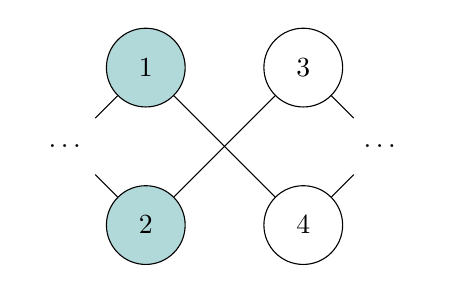
\begin{tikzpicture}[every node/.style={circle, draw, minimum size=1cm}]
			\node[draw=none] (dots1) at (0, 1) {\dots};
			\node[fill=teal!30] (1) at (1, 2) {1};
			\node[fill=teal!30] (2) at (1, 0) {2};
			\node (3) at (3, 2) {3};
			\node (4) at (3, 0) {4};
			\node[draw=none] (dots2) at (4, 1) {\dots};

			\draw (1) -- (4);
			\draw (2) -- (3);

			\draw (1) -- (dots1);
			\draw (2) -- (dots1);
			\draw (3) -- (dots2);
			\draw (4) -- (dots2);
		\end{tikzpicture}
		\caption{Separator in non-planar graph}
	\end{subfigure}
	\hfill
	\begin{subfigure}{0.45\linewidth}
		\centering
		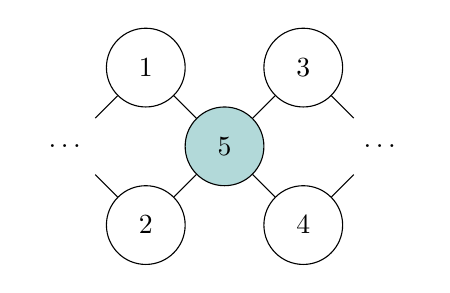
\begin{tikzpicture}[every node/.style={circle, draw, minimum size=1cm}]
			\node[draw=none] (dots1) at (0, 1) {\dots};
			\node (1) at (1, 2) {1};
			\node (2) at (1, 0) {2};
			\node (3) at (3, 2) {3};
			\node (4) at (3, 0) {4};
			\node[fill=teal!30] (5) at (2, 1) {5};
			\node[draw=none] (dots2) at (4, 1) {\dots};

			\draw (1) -- (5);
			\draw (2) -- (5);
			\draw (3) -- (5);
			\draw (4) -- (5);

			\draw (1) -- (dots1);
			\draw (2) -- (dots1);
			\draw (3) -- (dots2);
			\draw (4) -- (dots2);
		\end{tikzpicture}
		\caption{Better separator in planarized graph}
	\end{subfigure}
	\caption{Example of a separator, where a better separator can be found in the planarized graph.}
	\label{fig:planarization_reduces_separator}
\end{figure}

\begin{figure}
	\centering
	\begin{subfigure}{0.45\linewidth}
		\centering
		\begin{tikzpicture}[every node/.style={circle, draw, minimum size=1cm, node distance=1.5cm}]
			\node[fill=teal!30] (1) {1};
			\node[below right=of 1, fill=teal!30] (3) {3};
			\node[left=3cm of 3] (2) {2};
			\node[below left=of 3] (4) {4};

			\draw (1) -- (4);
			\draw (1) -- (2) -- (3);

			\node[right=of 1, draw=none] (dots1) {\dots};
			\node[right=of 4, draw=none] (dots4) {\dots};
			\draw (1) -- (dots1);
			\draw (4) -- (dots4);
			\draw (3) -- (dots4);
			\draw (3) -- (dots1);

			\draw[dashed] (-1, 1) -- (-1, -4.5);
		\end{tikzpicture}
		\caption{Separator in non-planar graph\newline}
	\end{subfigure}
	\hfill
	\begin{subfigure}{0.45\linewidth}
		\centering
		\begin{tikzpicture}[every node/.style={circle, draw, minimum size=1cm, node distance=1.5cm}]
			\node[fill=teal!30] (1) {1};
			\node[below right=of 1, fill=teal!30] (3) {3};
			\node[left=3cm of 3, fill=teal!5] (2) {2};
			\node[below left=of 3, fill=teal!5] (4) {4};
			\node[below= 0.75 of 1, fill=teal!5] (5) {5};

			\draw (1) -- (5);
			\draw (4) -- (5);
			\draw (5) -- (3);
			\draw (1) -- (2) -- (5);

			\node[right=of 1, draw=none] (dots1) {\dots};
			\node[right=of 4, draw=none] (dots4) {\dots};
			\draw (1) -- (dots1);
			\draw (4) -- (dots4);
			\draw (3) -- (dots4);
			\draw (3) -- (dots1);

			\draw[dashed] (-1, 1) -- (-1, -4.5);
		\end{tikzpicture}
		\caption{The separator of the original graph is not a separator in the planarized graph.}
	\end{subfigure}
	\caption{Example where the separator of the original graph is not a separator in the planarized graph.}
    \label{fig:planarization_increases_separator}
\end{figure}



\begin{figure}
	\centering
	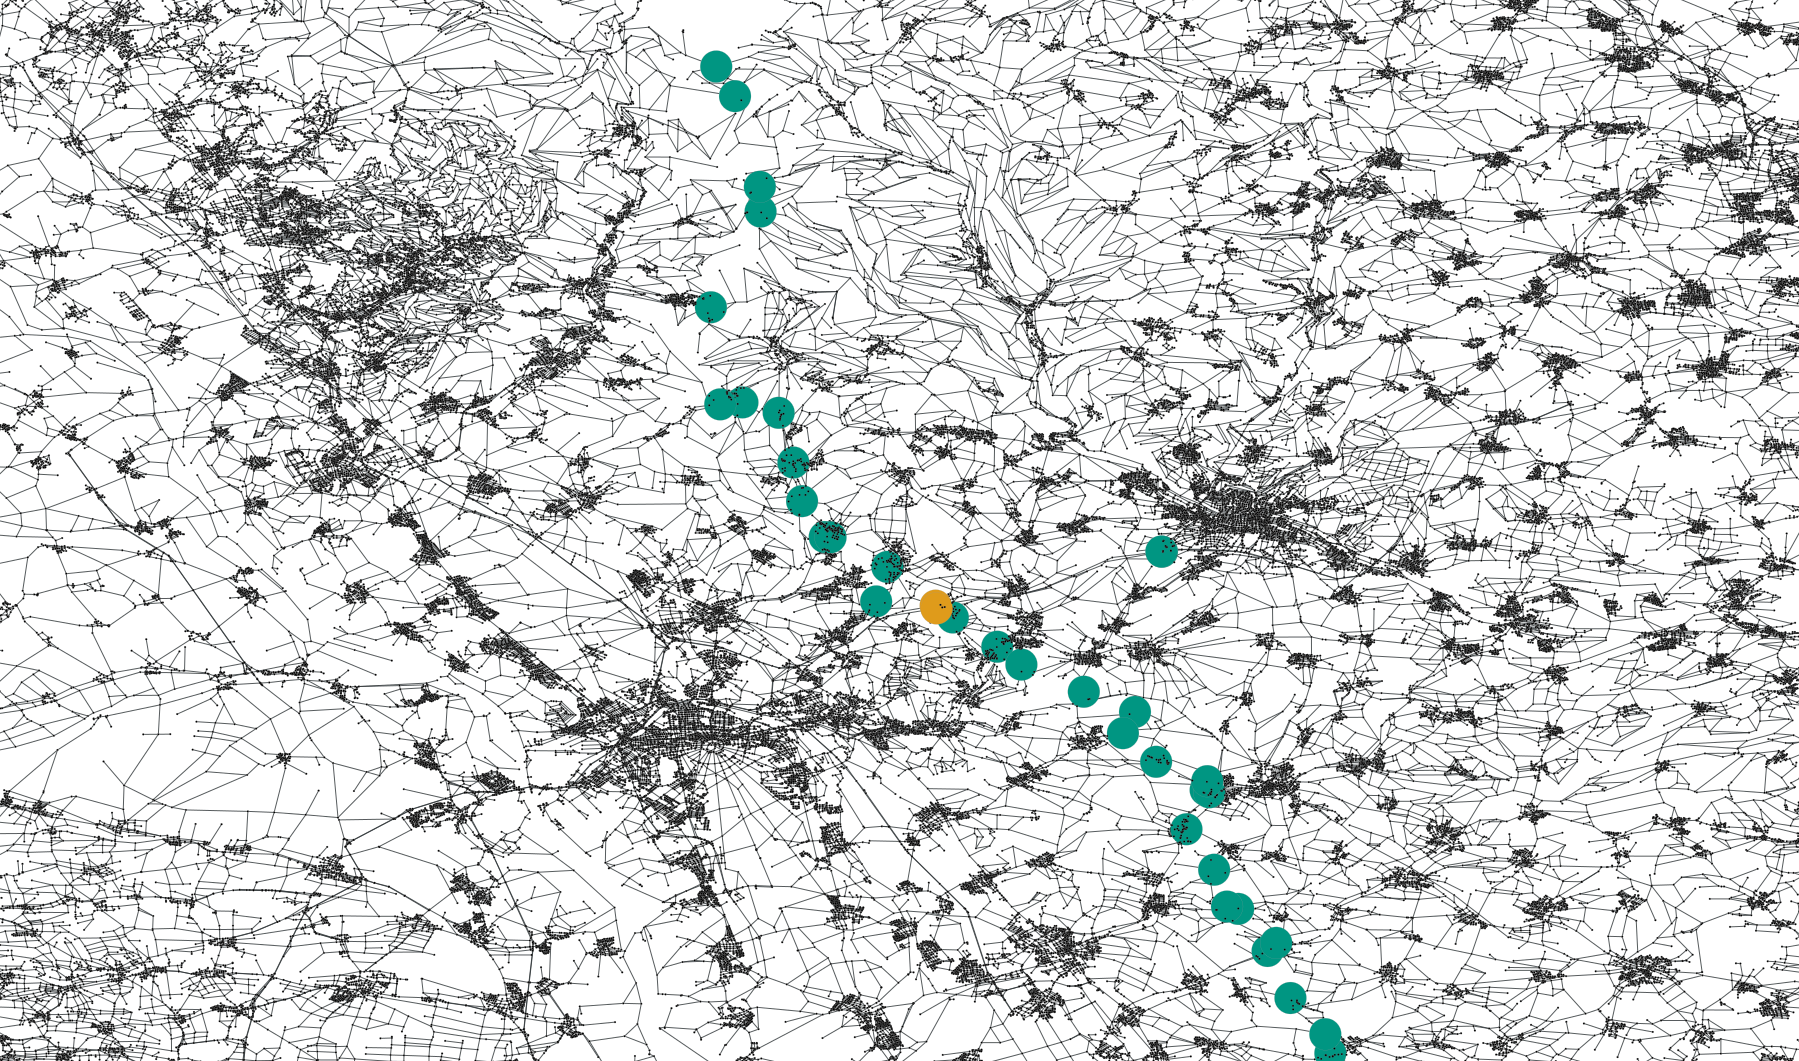
\includegraphics[width=0.8\linewidth]{graphics/karlsruhe_top_level_sep_extended_to_planar_wide.png}
	\caption{Visualization of a potential top-level separator for the road network of Karlsruhe.
		Vertices colored teal represent the separator nodes identified within the original, non-planar graph representation.
        Orange vertices (two almost overlapping ones) indicate the additional nodes required to establish a valid separator for the planarized version of the Karlsruhe road network.
		The single teal vertex located on the right side of the figure corresponds to a highway intersection.
		Although seemingly isolated in this view, its inclusion in the separator is necessary.}
	\label{fig:karlsruhe_planar_vs_non_planar}
\end{figure}

These findings highlight that the near-planar structure of road networks has
minimal impact on separator size, suggesting that such networks can typically
be analyzed as planar graphs.
